\section{Robustness to the target-set convention}
\label{sec:app_robustness}

Clauses \cone and \ctwo concern \plddt alone and should not be hostage to other panel members'
coverage. \tabref{tab:robustness} repeats the clause tests under three target-set conventions:
the intersection of targets covered by every panel method (used for all method comparisons),
\plddt's own coverage (used in \tabref{tab:clause}), and the full reference with targets absent
from \afdb scored as all-ordered. \caidthree has full AlphaFold coverage, so its last two rows
coincide. Sensitivity spans $0.51$--$0.63$; the pessimistic convention lowers it, and nothing
raises it near 0.8.

\begin{table}[h]
    \centering
    \small
    \resizebox{\textwidth}{!}{%
    \begin{tabular}{@{}llrrrrrrr@{}}
        \toprule
        \textbf{Reference set} & \textbf{Target set} & \textbf{$n$} & \textbf{Sens.} &
        \textbf{Sens $>$30} & \textbf{Sens $<$20} & \textbf{Spec.} & \textbf{\bacc} & \textbf{AUC} \\
        \midrule
        \multirow{3}{*}{\caidtwo \dpdb}
          & panel intersection & 240 & 0.576 & 0.598 & 0.393 & 0.988 & 0.782 & 0.932 \\
          & \plddt own coverage & 299 & 0.610 & 0.634 & 0.416 & 0.986 & 0.798 & 0.929 \\
          & all targets, missing $=$ ordered & 348 & 0.511 & 0.528 & 0.366 & 0.989 & 0.750 & 0.810 \\
        \midrule
        \multirow{3}{*}{\caidtwo \dnox}
          & panel intersection & 135 & 0.575 & 0.583 & 0.433 & 0.712 & 0.644 & 0.715 \\
          & \plddt own coverage & 173 & 0.620 & 0.630 & 0.429 & 0.673 & 0.646 & 0.695 \\
          & all targets, missing $=$ ordered & 210 & 0.511 & 0.520 & 0.332 & 0.788 & 0.649 & 0.692 \\
        \midrule
        \multirow{2}{*}{\caidthree \dpdb}
          & panel intersection & 261 & 0.551 & 0.583 & 0.331 & 0.987 & 0.769 & 0.943 \\
          & \plddt own coverage / all targets & 319 & 0.599 & 0.630 & 0.349 & 0.980 & 0.790 & 0.934 \\
        \midrule
        \multirow{2}{*}{\caidthree \dnox}
          & panel intersection & 161 & 0.588 & 0.608 & 0.250 & 0.835 & 0.712 & 0.833 \\
          & \plddt own coverage / all targets & 204 & 0.629 & 0.648 & 0.264 & 0.761 & 0.695 & 0.778 \\
        \bottomrule
    \end{tabular}}
    \caption{Clause tests under three target-set conventions. The conclusion for \cone is
    unchanged in all cases.}
    \label{tab:robustness}
\end{table}

\section{Region-level detection rates}
\label{sec:app_regions}

The folk rule is phrased about regions, so \tabref{tab:regiondetect} reports region-level
detection: a region counts as detected when at least a given fraction of its evaluated residues
is predicted disordered at the literal cut. The length ordering of \secref{sec:c4} survives at
every overlap criterion.

\begin{table}[h]
    \centering
    \small
    \resizebox{\textwidth}{!}{%
    \begin{tabular}{@{}lrrrrrrr@{}}
        \toprule
        \textbf{Reference set} & \textbf{Min overlap} & \textbf{Det.\ $<$20 aa} & \textbf{$n$} &
        \textbf{Det.\ 20--30 aa} & \textbf{$n$} & \textbf{Det.\ $>$30 aa} & \textbf{$n$} \\
        \midrule
        \multirow{3}{*}{\caidtwo \dpdb}
          & 0.25 & 0.737 & 118 & 0.797 & 64 & \textbf{0.869} & 153 \\
          & 0.50 & 0.661 & 118 & 0.719 & 64 & \textbf{0.797} & 153 \\
          & 0.75 & 0.576 & 118 & 0.625 & 64 & \textbf{0.641} & 153 \\
        \midrule
        \multirow{3}{*}{\caidtwo \dnox}
          & 0.25 & 0.871 & 31 & 0.808 & 26 & \textbf{0.932} & 117 \\
          & 0.50 & 0.806 & 31 & 0.769 & 26 & \textbf{0.863} & 117 \\
          & 0.75 & \textbf{0.774} & 31 & 0.654 & 26 & 0.701 & 117 \\
        \midrule
        \multirow{3}{*}{\caidthree \dpdb}
          & 0.25 & 0.772 & 136 & 0.797 & 64 & \textbf{0.907} & 172 \\
          & 0.50 & 0.647 & 136 & 0.750 & 64 & \textbf{0.831} & 172 \\
          & 0.75 & 0.544 & 136 & 0.547 & 64 & \textbf{0.686} & 172 \\
        \midrule
        \multirow{3}{*}{\caidthree \dnox}
          & 0.25 & 0.750 & 44 & 0.844 & 32 & \textbf{0.939} & 131 \\
          & 0.50 & 0.591 & 44 & 0.781 & 32 & \textbf{0.893} & 131 \\
          & 0.75 & 0.523 & 44 & 0.625 & 32 & \textbf{0.740} & 131 \\
        \bottomrule
    \end{tabular}}
    \caption{Region-level detection rate of \plddtrule by region length and overlap criterion.}
    \label{tab:regiondetect}
\end{table}

\section{Conditional information within \texorpdfstring{\plddt}{pLDDT} strata}
\label{sec:app_condinfo}

\tabref{tab:condinfo} reports, within each \plddt band, how well the solvent accessibility of the
same model separates disordered from ordered residues, together with the cross-validated logistic
probes of \secref{sec:c3}. Inside the $<$50 band --- where the confidence signal has saturated and
discriminates at AUC $0.44$--$0.63$ --- the geometry of the same model still reaches
$0.56$--$0.83$.

\begin{table}[h]
    \centering
    \small
    \begin{tabular}{@{}lrrrrrrr@{}}
        \toprule
        & \multicolumn{4}{c}{\textbf{AUC(RSA) within \plddt band}} & \multicolumn{3}{c}{\textbf{5-fold CV logistic probe}} \\
        \cmidrule(lr){2-5} \cmidrule(lr){6-8}
        \textbf{Reference set} & \textbf{0--50} & \textbf{50--70} & \textbf{70--90} & \textbf{90--100} &
        \textbf{\plddt} & \textbf{RSA} & \textbf{both} \\
        \midrule
        \caidtwo \dpdb   & 0.824 & 0.877 & 0.815 & 0.733 & 0.9263 & 0.9440 & \textbf{0.9490} \\
        \caidtwo \dnox   & 0.559 & 0.689 & 0.777 & 0.674 & 0.6888 & 0.7405 & \textbf{0.7431} \\
        \caidthree \dpdb & 0.829 & 0.901 & 0.818 & 0.773 & 0.9314 & 0.9488 & \textbf{0.9555} \\
        \caidthree \dnox & 0.621 & 0.829 & 0.799 & 0.754 & 0.7613 & \textbf{0.8267} & 0.8218 \\
        \bottomrule
    \end{tabular}
    \caption{Residual disorder signal in AlphaFold2 geometry, conditioned on confidence. Adding
    \plddt on top of RSA gains at most $+0.007$ AUC and loses $0.005$ on \caidthree \dnox, while
    adding RSA on top of \plddt gains $+0.023$ to $+0.065$.}
    \label{tab:condinfo}
\end{table}

\section{Calibration optimism}
\label{sec:app_optimism}

Our primary operating point selects each method's MCC-optimal threshold on the evaluation data.
\tabref{tab:optimism} quantifies the resulting optimism by repeated $5\times2$-fold
cross-validation over targets: the median gap is $0.20$--$0.66$ percentage points of balanced
accuracy, with a maximum of $3.0$\pp over 186 method\,$\times$\,dataset combinations. The
calibrated rankings in \secref{sec:ranking} are therefore not an artefact of tuning on the
evaluation data.

\begin{table}[h]
    \centering
    \small
    \resizebox{\textwidth}{!}{%
    \begin{tabular}{@{}lrrrrr@{}}
        \toprule
        \textbf{Reference set} & \textbf{$n$ methods} & \textbf{Median in-sample \bacc} &
        \textbf{Median CV \bacc} & \textbf{Median optimism (pp)} & \textbf{Max optimism (pp)} \\
        \midrule
        \caidtwo \dpdb   & 37 & 0.8175 & 0.8125 & 0.281 & 1.367 \\
        \caidtwo \dnox   & 37 & 0.7000 & 0.6848 & 0.663 & 3.036 \\
        \caidthree \dpdb & 56 & 0.8272 & 0.8255 & 0.196 & 1.691 \\
        \caidthree \dnox & 56 & 0.7625 & 0.7571 & 0.339 & 2.524 \\
        \bottomrule
    \end{tabular}}
    \caption{In-sample versus cross-validated calibrated balanced accuracy.}
    \label{tab:optimism}
\end{table}

\section{Full panel ranking}
\label{sec:app_ranking}

\Figref{fig:ranking} shows the calibrated, coverage-matched ranking of the whole panel on all
four reference sets, with \plddt and the AlphaFold-derived controls highlighted. \Figref{fig:calib}
shows the empirical probability of disorder as a function of \plddt bin, which is the graphical
form of \tabref{tab:calibration}.

\begin{figure}[h]
    \centering
    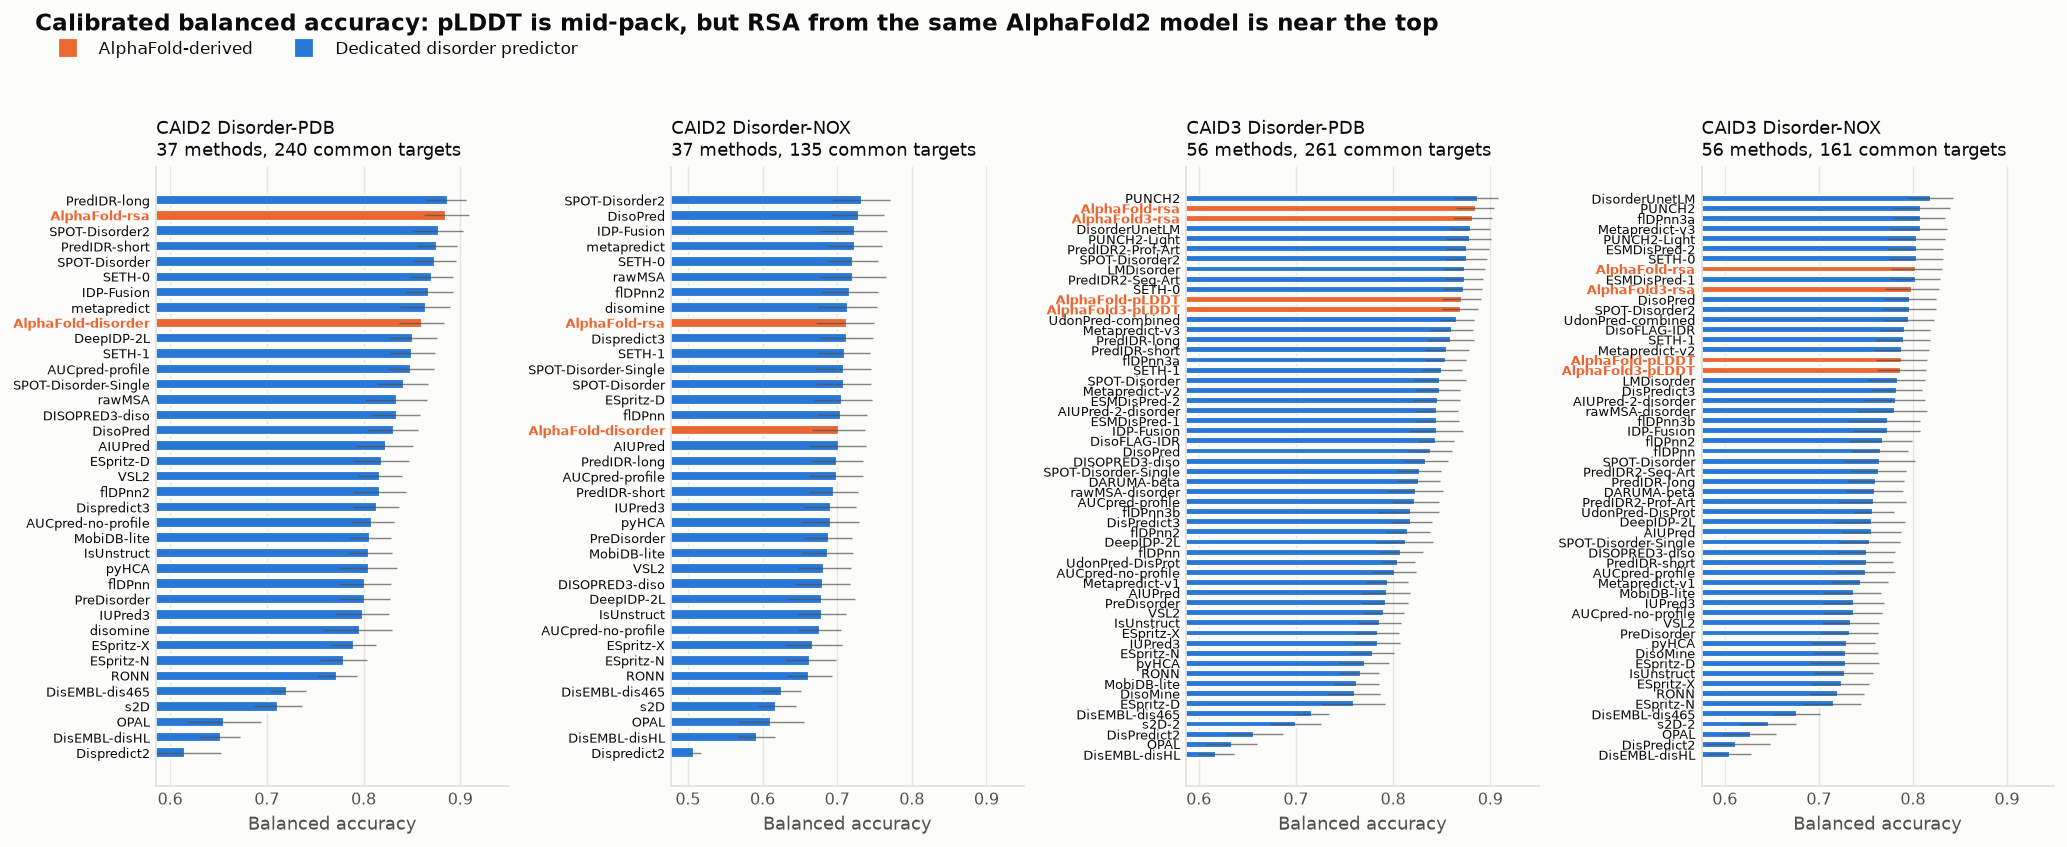
\includegraphics[width=0.92\linewidth]{figures/fig3_benchmark_ranking.png}
    \caption{Calibrated balanced accuracy of every panel method on the coverage-matched target
    sets. \plddt is mid-pack on all four references; \afrsa, read from the same coordinates, is
    consistently near the top.}
    \label{fig:ranking}
\end{figure}

\begin{figure}[h]
    \centering
    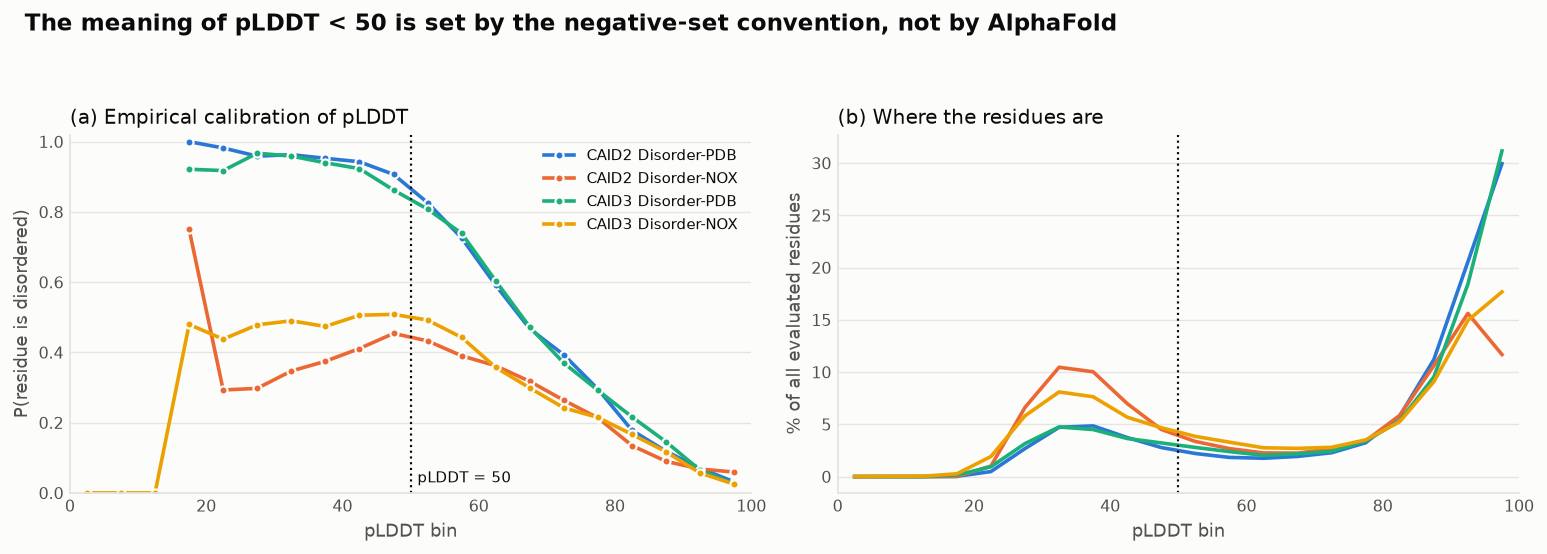
\includegraphics[width=0.92\linewidth]{figures/fig5_calibration.png}
    \caption{Empirical probability that a residue is annotated disordered, as a function of its
    \plddt bin. The curves for the two negative-set conventions are shifted by roughly a factor
    of two in precision at every bin, while the fraction of all disorder falling below \plddt 50
    is nearly identical.}
    \label{fig:calib}
\end{figure}
